\documentclass[tikz,border=2mm]{standalone}
\usepackage{tikz}
\usepackage{pgfplots}
\pgfplotsset{compat=1.18}

\begin{document}
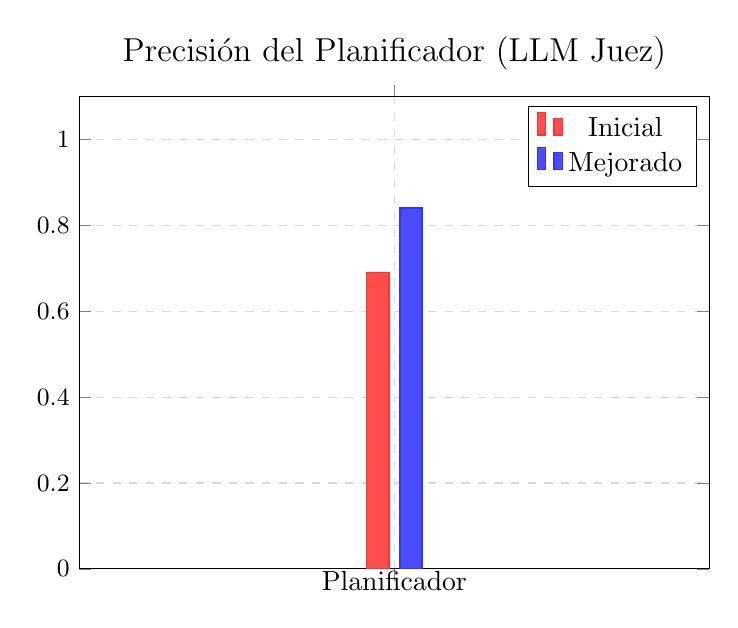
\begin{tikzpicture}
\begin{axis}[
    title={Precisión del Planificador (LLM Juez)},
    title style={font=\large},
    ylabel=,  
    xlabel=,
    ymin=0,
    ymax=1.1,
    ytick={0,0.2,0.4,0.6,0.8,1.0},
    enlarge x limits=0.8,
    ybar=4pt,
    bar width=8pt,
    symbolic x coords={Planificador},
    xtick={Planificador},
    x tick label style={rotate=0, anchor=center, font=\normalsize},
    yticklabel style={font=\small},
    width=8cm,
    height=6cm,
    grid=major,
    grid style={dashed, gray!30},
    tick label style={font=\small},
    scale only axis,
]
\addplot[
    fill=red!70,
    draw=red!80,
    line width=0.5pt
] coordinates {
    (Planificador, 0.69)
};
\addplot[
    fill=blue!70,
    draw=blue!80,
    line width=0.5pt
] coordinates {
    (Planificador, 0.84)
};
\legend{Inicial, Mejorado}
\end{axis}
\end{tikzpicture}
\end{document}
